\begin{evenBlock}{Triangle Passing with a Defender}
\textbf{Drill Description:}
        This drill is like the `Triangle Passing Drill' but incorporates a defender to improve the passing decision ability of the players.  The defender blocks one of the four lanes, if a pass is attempted on that lane the defender can block the pass.  If the passing team makes more than 2 touches, (uses the incorrect foot optional) for their first touch, the pass touches a cone or crosses into the box the offending player loses one of their lives 'a cone'.

        Give each passer 3 cones.  After the defender counts 10 passes they switch with the passer with the least amount of cones.

        This is a passing/possession drill not a defensive drill. The defense should never be able to win the ball.  This drill is about watching the defenders position and deciding on a passing location before the pass is made, so the first touch can place the ball in a location to make a quick pass and beat the defender.

        Variation add a passer to each cone to eliminate the movement and focus on the passing location if the receiving player movement is causing issues.
\begin{minipage}[t]{\linewidth}
    \begin{minipage}{.3\linewidth} % Left column and width
        \centering
        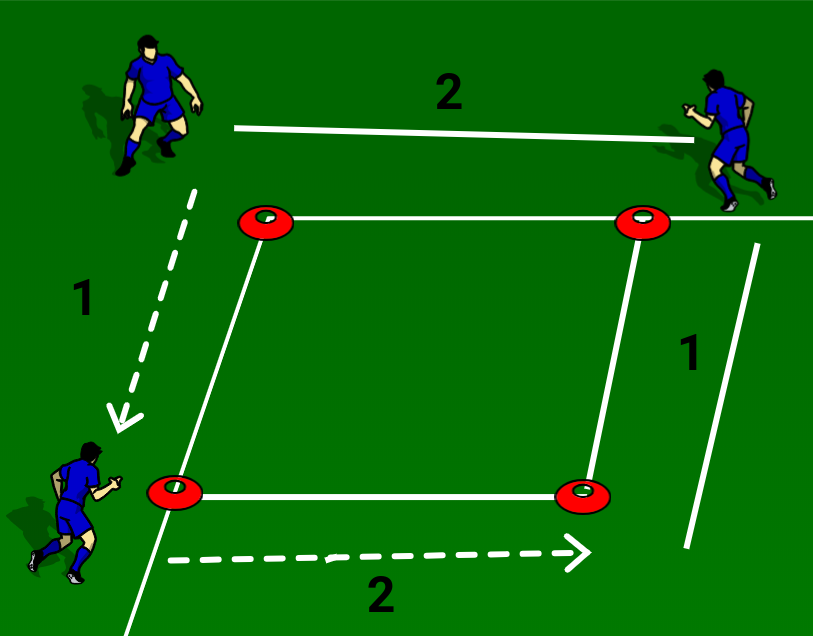
\includegraphics[width=\textwidth]{../img/Trimmed/Triangle_Passing_3P_mini}
    \end{minipage}
    \hspace{0.05\linewidth}
    \begin{minipage}{.6\linewidth} % Left column and width
        \begin{enumerate}
            \setlength{\itemsep}{0pt}
            \setlength{\parskip}{0pt}
            \setlength{\parsep}{0pt}
            \item All players stand `open' so they can see the other two players.
            \item The player receiving the ball should move his body so he receives the ball on the correct foot (first touch) then passes it to the next `open' player.
            \item  Four opposite colored cones should be placed between each corner cone.  The defender can block the passing lane if he is positioned such that his body is over the cone.  If the pass it attempted in that direction he can block the pass.  If successful the passer loses a `life' (drops one of his cones).
        \end{enumerate}
    \end{minipage}
\end{minipage}
\raggedright
    \textbf{Coaching Points:}
    \begin{itemize}
        \setlength{\itemsep}{0pt}
        \setlength{\parskip}{0pt}
        \setlength{\parsep}{0pt}
        \item Explain the first touch with the correct foot is the most important part.
        \item The touch should place the ball one step away from the player so they can step into and make a strong pass.
        \item Watch the defender and decide before the pass is made where the next pass should go.  The receiver must also be moving and watching the defenders movement so he can receive the pass and then play the ball to the next position correctly.
    \end{itemize}

\end{evenBlock}